
\tikzstyle{hidden_neuron}=[circle,draw=blue!50,fill=cyan!10,thick,minimum size=4mm]
\begin{tikzpicture}
\newcommand*{\xpos}{10}
\newcommand*{\rectstarty}{1.3}
\newcommand*{\rectendy}{4}

\renewcommand*{\xpos}{20}
\draw[rounded corners,fill=cyan!20] (\xpos-0.4, \rectstarty) rectangle (\xpos+0.4, \rectendy) {};
\node (N) at (\xpos,2) {};
\node[hidden_neuron] (N1) at (\xpos,1+1*0.65) {};
\node[hidden_neuron] (N2) at (\xpos,1+2*0.65) {};
\node[hidden_neuron] (N3) at (\xpos,1+3*0.65) {};
\node[hidden_neuron] (N4) at (\xpos,1+4*0.65) {};
\node (N) at (\xpos,1) {\small{$z \sim N(0,I)$}};

\draw[->,thick,black] (\xpos+0.4,2.7) -- (\xpos+0.4+1.5,2.7);

\draw[rounded corners,fill=green!12] (\xpos+0.4+1.5, \rectstarty+1) rectangle (\xpos+0.4+5.5, \rectendy-0.7) {};
\node (N) at (\xpos+0.4+2+1.5,\rectstarty+0.5+1) {\small{Complex Transformation}};

\draw[->,thick,black] (\xpos+0.4+5.5, 2.7) -- (\xpos+0.4+6+1, 2.7);
\node (N) at (\xpos+0.4+6+1.7, 2.7) {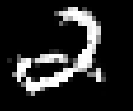
\includegraphics[scale=0.3]{images/sample1.png}};
\node (N) at (\xpos+0.4+6+1.7,1.7) {\textcolor{red}{\small{Sample Generated}}};

\end{tikzpicture}